\section{Evaluation}\label{evaluation}

Difficult to train binarized model~\cite{AAAI1714619}

\begin{table}[!htb]
\begin{center}
\renewcommand\arraystretch{1.5}
\fontsize{6.7pt}{6.7pt}\selectfont
\begin{tabular}{|c|c|c|c|c|}
\hline
\multicolumn{5}{|c|}{\textbf{CIFAR10}} \\
\hline
\multicolumn{2}{|c|}{\textbf{Architecture}} & \textbf{Train}  & \textbf{Test}  & \textbf{Inference}  \\
 \multicolumn{2}{|c|}{} & \textbf{Accuracy} & \textbf{Accuracy} & \textbf{Accuracy}  \\
\hline
\multirow{2}{*}{NiN} & Full Precision & 98.16\% & 86.16\% & \cellcolor{red!25}56.69\% \\
& Binary Precision & 81.93\% & 78.74\% & \cellcolor{green!25}51.76\% \\
\hline
\multirow{2}{*}{AlexNet} & Full Precision & 97.86\% & 80.34\% & \cellcolor{red!25}60.40\% \\
& Binary Precision & 68.62\% & 66.8\% & \cellcolor{green!25}51.40\% \\
\hline
\multirow{2}{*}{VGG16} & Full Precision & 99.58\% & 88.95\% & \cellcolor{red!25}58.70\%\\
& Binary Precision & 79.67\% & 74.64\% & \cellcolor{green!25}52.65\%\\
\hline
\end{tabular}
\end{center}
\caption{Reducing the precision of models lowers the membership privacy leakage through membership inference attacks but at the cost of accuracy}
\label{fmnist_quantize}
\end{table}


%\pgfplotsset{footnotesize,height=5.5cm,width=0.35\textwidth}
% \pgfplotsset{footnotesize,samples=10}

\begin{figure*}[ht!]
\begin{center}% note that \centering uses less vspace...
\resizebox{2\columnwidth}{!}{%
\begin{tabular}{lllll}


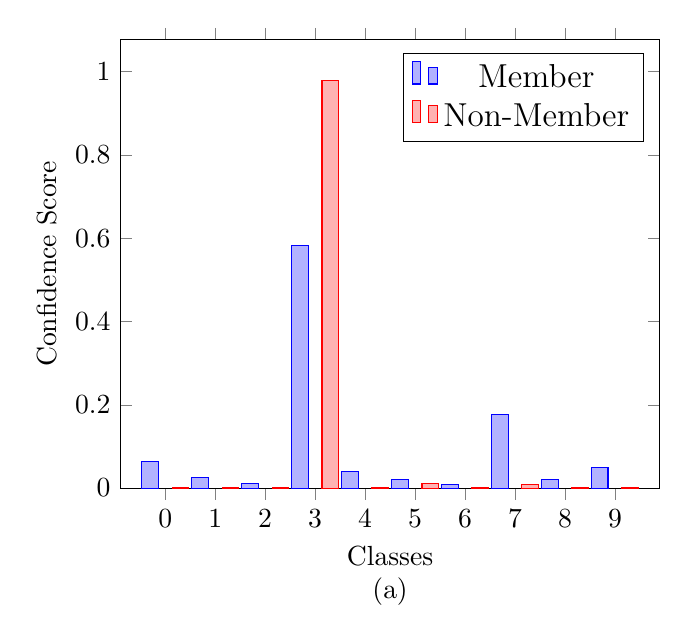
\begin{tikzpicture}
\begin{axis}[title={(a)},
title style={at={(0.5,0)},anchor=north,yshift=-35},
ylabel=Confidence Score,
xlabel=Classes,
legend style={font=\large},
legend pos =  north east,
ybar=5pt,% configures ‘bar shift’
bar width=6pt,
xtick={0,1,2,3,4,5,6,7,8,9},
ymin=0
]

\addplot
coordinates {(0,0.06327114254236221) (1,0.025417674332857132) (2,0.011714407242834568) (3,0.5831579566001892) (4,0.04046289622783661) (5,0.02152826450765133) (6,0.00799587182700634) (7,0.1768314242362976) (8,0.021124042570590973) (9,0.04849636182188988)};
\addplot
coordinates {(0,0.0010145490523427725) (1,0.00030558116850443184) (2,0.0008154626120813191) (3,0.9787409901618958) (4,0.00029880856163799763) (5,0.010064681060612202) (6,0.00022722511494066566) (7,0.007986118085682392) (8,0.00020130971097387373) (9,0.00034515938023105264)};

\legend{Member,Non-Member}
\end{axis}
\end{tikzpicture} &


%
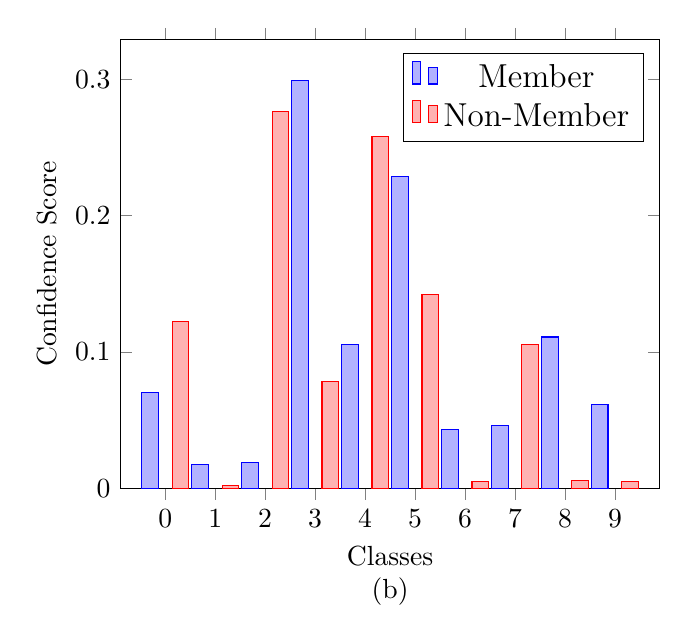
\begin{tikzpicture}
\begin{axis}[title={(b)},
title style={at={(0.5,0)},anchor=north,yshift=-35},
ylabel=Confidence Score,
xlabel=Classes,
xtick={0,1,2,3,4,5,6,7,8,9},
legend style={font=\large},
legend pos =  north east,
ybar=5pt,% configures ‘bar shift’
bar width=6pt,
ymin=0
]

\addplot
coordinates {(0,0.07000309228897095) (1,0.017400363460183144) (2,0.019030457362532616) (3,0.29907193779945374) (4,0.10515590757131577) (5,0.22833536565303802) (6,0.04266407713294029) (7,0.04584269970655441) (8,0.11086355894804001) (9,0.061632607132196426)};
\addplot
coordinates {(0,0.12253900617361069) (1,0.0015809950418770313) (2,0.27642616629600525) (3,0.07850959151983261) (4,0.2582301199436188) (5,0.14231687784194946) (6,0.004606064409017563) (7,0.10550655424594879) (8,0.005763859022408724) (9,0.004520699847489595)};

\legend{Member,Non-Member}
\end{axis}
\end{tikzpicture} &





%
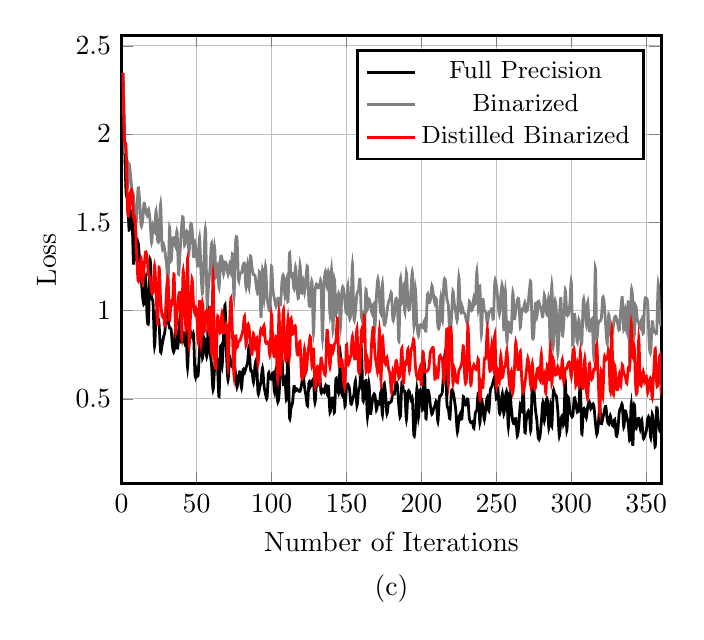
\begin{tikzpicture}
\begin{axis}[title={(c)},
title style={at={(0.5,0)},anchor=north,yshift=-35},
line width=1.0pt,
legend style={font=\small},
legend pos =  north east,
legend entries={Full Precision, Binarized, Distilled Binarized},
ylabel={Loss},
xmin=0,
xmax=360,
xlabel={Number of Iterations},
% extra x ticks={1,10,...,400},
% extra y ticks={0,0.5,...,10},
% extra y tick labels={},
% extra x tick labels={},
% extra x tick style={grid=major},
% extra y tick style={grid=major},
grid=major
]
\addplot[
    color=black,
    solid,
    smooth
    ]
    coordinates {
    ( 1 , 2.302968 )
    ( 2 , 1.939443 )
    ( 3 , 1.667299 )
    ( 4 , 1.652660 )
    ( 5 , 1.455838 )
    ( 6 , 1.559521 )
    ( 7 , 1.526025 )
    ( 8 , 1.260517 )
    ( 9 , 1.503018 )
    ( 10 , 1.285601 )
    ( 11 , 1.384281 )
    ( 12 , 1.286194 )
    ( 13 , 1.191418 )
    ( 14 , 1.079983 )
    ( 15 , 1.039906 )
    ( 16 , 1.188020 )
    ( 17 , 0.963824 )
    ( 18 , 0.943251 )
    ( 19 , 1.289535 )
    ( 20 , 1.082280 )
    ( 21 , 1.037991 )
    ( 22 , 0.799126 )
    ( 23 , 0.983668 )
    ( 24 , 0.966282 )
    ( 25 , 0.922792 )
    ( 26 , 0.765660 )
    ( 27 , 0.803365 )
    ( 28 , 0.850827 )
    ( 29 , 0.893062 )
    ( 30 , 1.063586 )
    ( 31 , 0.948933 )
    ( 32 , 0.901259 )
    ( 33 , 0.895251 )
    ( 34 , 0.794324 )
    ( 35 , 0.769924 )
    ( 36 , 0.899247 )
    ( 37 , 0.787751 )
    ( 38 , 0.831077 )
    ( 39 , 0.962390 )
    ( 40 , 0.821883 )
    ( 41 , 0.863004 )
    ( 42 , 0.818929 )
    ( 43 , 0.880331 )
    ( 44 , 0.676965 )
    ( 45 , 0.891206 )
    ( 46 , 0.876807 )
    ( 47 , 0.854072 )
    ( 48 , 0.860776 )
    ( 49 , 0.631650 )
    ( 50 , 0.662787 )
    ( 51 , 0.630878 )
    ( 52 , 0.778465 )
    ( 53 , 0.900262 )
    ( 54 , 0.731535 )
    ( 55 , 0.845547 )
    ( 56 , 0.785181 )
    ( 57 , 0.748590 )
    ( 58 , 0.986032 )
    ( 59 , 0.774422 )
    ( 60 , 0.691421 )
    ( 61 , 0.551147 )
    ( 62 , 0.668453 )
    ( 63 , 0.759031 )
    ( 64 , 0.673677 )
    ( 65 , 0.512989 )
    ( 66 , 0.796980 )
    ( 67 , 0.681779 )
    ( 68 , 0.851441 )
    ( 69 , 1.030697 )
    ( 70 , 0.751324 )
    ( 71 , 0.606460 )
    ( 72 , 0.733667 )
    ( 73 , 0.701998 )
    ( 74 , 0.680291 )
    ( 75 , 0.707206 )
    ( 76 , 0.645020 )
    ( 77 , 0.566519 )
    ( 78 , 0.622747 )
    ( 79 , 0.651569 )
    ( 80 , 0.560384 )
    ( 81 , 0.663585 )
    ( 82 , 0.648072 )
    ( 83 , 0.676273 )
    ( 84 , 0.701089 )
    ( 85 , 0.797614 )
    ( 86 , 0.665663 )
    ( 87 , 0.657626 )
    ( 88 , 0.592905 )
    ( 89 , 0.687644 )
    ( 90 , 0.712525 )
    ( 91 , 0.533854 )
    ( 92 , 0.557828 )
    ( 93 , 0.599991 )
    ( 94 , 0.673825 )
    ( 95 , 0.575448 )
    ( 96 , 0.526772 )
    ( 97 , 0.505667 )
    ( 98 , 0.643386 )
    ( 99 , 0.620009 )
    ( 100 , 0.610189 )
    ( 101 , 0.647692 )
    ( 102 , 0.539143 )
    ( 103 , 0.667260 )
    ( 104 , 0.489376 )
    ( 105 , 0.518314 )
    ( 106 , 0.676982 )
    ( 107 , 0.727331 )
    ( 108 , 0.581430 )
    ( 109 , 0.618056 )
    ( 110 , 0.500167 )
    ( 111 , 0.785589 )
    ( 112 , 0.399176 )
    ( 113 , 0.447618 )
    ( 114 , 0.475429 )
    ( 115 , 0.570146 )
    ( 116 , 0.544356 )
    ( 117 , 0.555152 )
    ( 118 , 0.546433 )
    ( 119 , 0.542349 )
    ( 120 , 0.577833 )
    ( 121 , 0.639318 )
    ( 122 , 0.567917 )
    ( 123 , 0.517693 )
    ( 124 , 0.460981 )
    ( 125 , 0.593507 )
    ( 126 , 0.570267 )
    ( 127 , 0.597812 )
    ( 128 , 0.598578 )
    ( 129 , 0.478810 )
    ( 130 , 0.586665 )
    ( 131 , 0.579736 )
    ( 132 , 0.659663 )
    ( 133 , 0.538597 )
    ( 134 , 0.549711 )
    ( 135 , 0.537823 )
    ( 136 , 0.572637 )
    ( 137 , 0.534132 )
    ( 138 , 0.570913 )
    ( 139 , 0.422553 )
    ( 140 , 0.488932 )
    ( 141 , 0.504971 )
    ( 142 , 0.423515 )
    ( 143 , 0.614434 )
    ( 144 , 0.564107 )
    ( 145 , 0.541557 )
    ( 146 , 0.744249 )
    ( 147 , 0.522557 )
    ( 148 , 0.606243 )
    ( 149 , 0.458936 )
    ( 150 , 0.558472 )
    ( 151 , 0.581740 )
    ( 152 , 0.556220 )
    ( 153 , 0.470633 )
    ( 154 , 0.493428 )
    ( 155 , 0.524618 )
    ( 156 , 0.601933 )
    ( 157 , 0.460702 )
    ( 158 , 0.542096 )
    ( 159 , 0.583347 )
    ( 160 , 0.778570 )
    ( 161 , 0.497549 )
    ( 162 , 0.533701 )
    ( 163 , 0.603471 )
    ( 164 , 0.397012 )
    ( 165 , 0.583966 )
    ( 166 , 0.417388 )
    ( 167 , 0.471393 )
    ( 168 , 0.520279 )
    ( 169 , 0.520528 )
    ( 170 , 0.437146 )
    ( 171 , 0.482065 )
    ( 172 , 0.469343 )
    ( 173 , 0.539111 )
    ( 174 , 0.408798 )
    ( 175 , 0.585470 )
    ( 176 , 0.532898 )
    ( 177 , 0.415162 )
    ( 178 , 0.476431 )
    ( 179 , 0.477853 )
    ( 180 , 0.486712 )
    ( 181 , 0.538571 )
    ( 182 , 0.526860 )
    ( 183 , 0.590460 )
    ( 184 , 0.575449 )
    ( 185 , 0.451290 )
    ( 186 , 0.401073 )
    ( 187 , 0.596629 )
    ( 188 , 0.545198 )
    ( 189 , 0.532833 )
    ( 190 , 0.382534 )
    ( 191 , 0.532536 )
    ( 192 , 0.539632 )
    ( 193 , 0.492966 )
    ( 194 , 0.496653 )
    ( 195 , 0.291686 )
    ( 196 , 0.359933 )
    ( 197 , 0.558284 )
    ( 198 , 0.393615 )
    ( 199 , 0.546782 )
    ( 200 , 0.507714 )
    ( 201 , 0.441790 )
    ( 202 , 0.694662 )
    ( 203 , 0.387495 )
    ( 204 , 0.539195 )
    ( 205 , 0.534799 )
    ( 206 , 0.460438 )
    ( 207 , 0.412882 )
    ( 208 , 0.439468 )
    ( 209 , 0.461498 )
    ( 210 , 0.484441 )
    ( 211 , 0.371391 )
    ( 212 , 0.505832 )
    ( 213 , 0.518648 )
    ( 214 , 0.544090 )
    ( 215 , 0.680713 )
    ( 216 , 0.751645 )
    ( 217 , 0.478645 )
    ( 218 , 0.442678 )
    ( 219 , 0.387577 )
    ( 220 , 0.538398 )
    ( 221 , 0.543274 )
    ( 222 , 0.495477 )
    ( 223 , 0.428225 )
    ( 224 , 0.311347 )
    ( 225 , 0.386528 )
    ( 226 , 0.415797 )
    ( 227 , 0.386841 )
    ( 228 , 0.512556 )
    ( 229 , 0.467811 )
    ( 230 , 0.469653 )
    ( 231 , 0.497145 )
    ( 232 , 0.386810 )
    ( 233 , 0.365984 )
    ( 234 , 0.370858 )
    ( 235 , 0.334157 )
    ( 236 , 0.421482 )
    ( 237 , 0.437231 )
    ( 238 , 0.533400 )
    ( 239 , 0.363779 )
    ( 240 , 0.499905 )
    ( 241 , 0.448234 )
    ( 242 , 0.381877 )
    ( 243 , 0.457827 )
    ( 244 , 0.508316 )
    ( 245 , 0.432367 )
    ( 246 , 0.550766 )
    ( 247 , 0.567483 )
    ( 248 , 0.600920 )
    ( 249 , 0.619330 )
    ( 250 , 0.501078 )
    ( 251 , 0.563693 )
    ( 252 , 0.420956 )
    ( 253 , 0.452368 )
    ( 254 , 0.529415 )
    ( 255 , 0.413688 )
    ( 256 , 0.507326 )
    ( 257 , 0.534332 )
    ( 258 , 0.340995 )
    ( 259 , 0.533992 )
    ( 260 , 0.445496 )
    ( 261 , 0.371866 )
    ( 262 , 0.357937 )
    ( 263 , 0.387621 )
    ( 264 , 0.290543 )
    ( 265 , 0.351936 )
    ( 266 , 0.467249 )
    ( 267 , 0.429069 )
    ( 268 , 0.564726 )
    ( 269 , 0.309757 )
    ( 270 , 0.382020 )
    ( 271 , 0.423434 )
    ( 272 , 0.425730 )
    ( 273 , 0.322237 )
    ( 274 , 0.597025 )
    ( 275 , 0.560745 )
    ( 276 , 0.445284 )
    ( 277 , 0.378794 )
    ( 278 , 0.276946 )
    ( 279 , 0.282341 )
    ( 280 , 0.366811 )
    ( 281 , 0.478299 )
    ( 282 , 0.375445 )
    ( 283 , 0.480307 )
    ( 284 , 0.493695 )
    ( 285 , 0.336665 )
    ( 286 , 0.462213 )
    ( 287 , 0.346743 )
    ( 288 , 0.541349 )
    ( 289 , 0.522342 )
    ( 290 , 0.514670 )
    ( 291 , 0.430172 )
    ( 292 , 0.289797 )
    ( 293 , 0.371195 )
    ( 294 , 0.405113 )
    ( 295 , 0.357373 )
    ( 296 , 0.603785 )
    ( 297 , 0.321793 )
    ( 298 , 0.506746 )
    ( 299 , 0.432704 )
    ( 300 , 0.405093 )
    ( 301 , 0.403066 )
    ( 302 , 0.504766 )
    ( 303 , 0.473787 )
    ( 304 , 0.425059 )
    ( 305 , 0.450767 )
    ( 306 , 0.582399 )
    ( 307 , 0.300974 )
    ( 308 , 0.433699 )
    ( 309 , 0.439344 )
    ( 310 , 0.394054 )
    ( 311 , 0.458976 )
    ( 312 , 0.482490 )
    ( 313 , 0.442764 )
    ( 314 , 0.467489 )
    ( 315 , 0.462829 )
    ( 316 , 0.372411 )
    ( 317 , 0.298418 )
    ( 318 , 0.353107 )
    ( 319 , 0.452360 )
    ( 320 , 0.359912 )
    ( 321 , 0.388992 )
    ( 322 , 0.428388 )
    ( 323 , 0.456512 )
    ( 324 , 0.380230 )
    ( 325 , 0.357444 )
    ( 326 , 0.403996 )
    ( 327 , 0.361251 )
    ( 328 , 0.344514 )
    ( 329 , 0.381908 )
    ( 330 , 0.289464 )
    ( 331 , 0.320182 )
    ( 332 , 0.425570 )
    ( 333 , 0.448104 )
    ( 334 , 0.466504 )
    ( 335 , 0.340016 )
    ( 336 , 0.430965 )
    ( 337 , 0.396781 )
    ( 338 , 0.356925 )
    ( 339 , 0.267577 )
    ( 340 , 0.468913 )
    ( 341 , 0.233512 )
    ( 342 , 0.466996 )
    ( 343 , 0.332996 )
    ( 344 , 0.367131 )
    ( 345 , 0.389329 )
    ( 346 , 0.330957 )
    ( 347 , 0.378960 )
    ( 348 , 0.278310 )
    ( 349 , 0.290548 )
    ( 350 , 0.316687 )
    ( 351 , 0.388542 )
    ( 352 , 0.388174 )
    ( 353 , 0.279368 )
    ( 354 , 0.412089 )
    ( 355 , 0.335098 )
    ( 356 , 0.229976 )
    ( 357 , 0.449180 )
    ( 358 , 0.374953 )
    ( 359 , 0.321231 )
    ( 360 , 0.348795 )
      };

      \addplot[
          color=gray,
          solid,
          smooth
          ]
          coordinates {
          ( 1 , 2.346761 )
  ( 2 , 1.926266 )
  ( 3 , 1.885543 )
  ( 4 , 1.695635 )
  ( 5 , 1.828619 )
  ( 6 , 1.763135 )
  ( 7 , 1.675170 )
  ( 8 , 1.648822 )
  ( 9 , 1.501599 )
  ( 10 , 1.517566 )
  ( 11 , 1.694481 )
  ( 12 , 1.630272 )
  ( 13 , 1.482632 )
  ( 14 , 1.509774 )
  ( 15 , 1.607969 )
  ( 16 , 1.573090 )
  ( 17 , 1.538904 )
  ( 18 , 1.573854 )
  ( 19 , 1.506782 )
  ( 20 , 1.384800 )
  ( 21 , 1.485137 )
  ( 22 , 1.445732 )
  ( 23 , 1.566089 )
  ( 24 , 1.400355 )
  ( 25 , 1.410617 )
  ( 26 , 1.602641 )
  ( 27 , 1.363793 )
  ( 28 , 1.374451 )
  ( 29 , 1.327962 )
  ( 30 , 1.259157 )
  ( 31 , 1.158507 )
  ( 32 , 1.471694 )
  ( 33 , 1.281064 )
  ( 34 , 1.395380 )
  ( 35 , 1.413245 )
  ( 36 , 1.364599 )
  ( 37 , 1.446778 )
  ( 38 , 1.205966 )
  ( 39 , 1.332203 )
  ( 40 , 1.474646 )
  ( 41 , 1.530147 )
  ( 42 , 1.370293 )
  ( 43 , 1.436183 )
  ( 44 , 1.444681 )
  ( 45 , 1.332167 )
  ( 46 , 1.484209 )
  ( 47 , 1.465831 )
  ( 48 , 1.305787 )
  ( 49 , 1.380785 )
  ( 50 , 1.305335 )
  ( 51 , 1.252715 )
  ( 52 , 1.414409 )
  ( 53 , 1.208195 )
  ( 54 , 1.097216 )
  ( 55 , 1.304714 )
  ( 56 , 1.456459 )
  ( 57 , 1.040485 )
  ( 58 , 1.141915 )
  ( 59 , 1.240699 )
  ( 60 , 1.379954 )
  ( 61 , 1.174325 )
  ( 62 , 1.360094 )
  ( 63 , 1.193203 )
  ( 64 , 1.246328 )
  ( 65 , 1.128607 )
  ( 66 , 1.297393 )
  ( 67 , 1.293353 )
  ( 68 , 1.207303 )
  ( 69 , 1.274779 )
  ( 70 , 1.260201 )
  ( 71 , 1.205472 )
  ( 72 , 1.257582 )
  ( 73 , 1.209281 )
  ( 74 , 1.320339 )
  ( 75 , 1.081225 )
  ( 76 , 1.379258 )
  ( 77 , 1.403371 )
  ( 78 , 1.173059 )
  ( 79 , 1.210906 )
  ( 80 , 1.212522 )
  ( 81 , 1.256900 )
  ( 82 , 1.261412 )
  ( 83 , 1.132829 )
  ( 84 , 1.261608 )
  ( 85 , 1.130152 )
  ( 86 , 1.307679 )
  ( 87 , 1.242157 )
  ( 88 , 1.203381 )
  ( 89 , 1.197875 )
  ( 90 , 1.127777 )
  ( 91 , 1.099596 )
  ( 92 , 1.218491 )
  ( 93 , 0.959279 )
  ( 94 , 1.230520 )
  ( 95 , 1.063139 )
  ( 96 , 1.248715 )
  ( 97 , 1.083069 )
  ( 98 , 1.019647 )
  ( 99 , 1.012220 )
  ( 100 , 1.250834 )
  ( 101 , 1.113485 )
  ( 102 , 1.065619 )
  ( 103 , 1.023666 )
  ( 104 , 1.063910 )
  ( 105 , 1.067258 )
  ( 106 , 1.032276 )
  ( 107 , 1.165910 )
  ( 108 , 1.197135 )
  ( 109 , 1.079468 )
  ( 110 , 1.176466 )
  ( 111 , 1.049984 )
  ( 112 , 1.325067 )
  ( 113 , 1.198396 )
  ( 114 , 1.209702 )
  ( 115 , 1.122866 )
  ( 116 , 1.246204 )
  ( 117 , 1.130638 )
  ( 118 , 1.070367 )
  ( 119 , 1.258520 )
  ( 120 , 1.100373 )
  ( 121 , 1.169035 )
  ( 122 , 1.103153 )
  ( 123 , 1.187527 )
  ( 124 , 1.249404 )
  ( 125 , 1.039255 )
  ( 126 , 1.043600 )
  ( 127 , 1.163061 )
  ( 128 , 0.866229 )
  ( 129 , 1.100545 )
  ( 130 , 1.150101 )
  ( 131 , 1.129426 )
  ( 132 , 1.129657 )
  ( 133 , 1.159651 )
  ( 134 , 0.838983 )
  ( 135 , 1.136622 )
  ( 136 , 1.221408 )
  ( 137 , 1.139824 )
  ( 138 , 1.213746 )
  ( 139 , 0.979337 )
  ( 140 , 1.232616 )
  ( 141 , 0.885131 )
  ( 142 , 1.174824 )
  ( 143 , 0.979129 )
  ( 144 , 1.055910 )
  ( 145 , 1.090147 )
  ( 146 , 0.904567 )
  ( 147 , 1.113498 )
  ( 148 , 1.125462 )
  ( 149 , 1.049405 )
  ( 150 , 0.985949 )
  ( 151 , 1.139380 )
  ( 152 , 0.959967 )
  ( 153 , 1.000041 )
  ( 154 , 1.263282 )
  ( 155 , 0.956478 )
  ( 156 , 0.995327 )
  ( 157 , 1.096886 )
  ( 158 , 1.111590 )
  ( 159 , 1.176757 )
  ( 160 , 0.962864 )
  ( 161 , 0.977689 )
  ( 162 , 0.922844 )
  ( 163 , 1.120963 )
  ( 164 , 1.009984 )
  ( 165 , 1.063984 )
  ( 166 , 1.032832 )
  ( 167 , 0.987173 )
  ( 168 , 1.035523 )
  ( 169 , 0.903309 )
  ( 170 , 1.083587 )
  ( 171 , 1.178625 )
  ( 172 , 1.068447 )
  ( 173 , 0.984077 )
  ( 174 , 1.152232 )
  ( 175 , 0.932497 )
  ( 176 , 0.932060 )
  ( 177 , 0.994724 )
  ( 178 , 1.047627 )
  ( 179 , 1.068406 )
  ( 180 , 1.097718 )
  ( 181 , 0.946308 )
  ( 182 , 0.981098 )
  ( 183 , 1.067997 )
  ( 184 , 1.027874 )
  ( 185 , 0.826300 )
  ( 186 , 1.179658 )
  ( 187 , 1.052969 )
  ( 188 , 1.142715 )
  ( 189 , 0.991129 )
  ( 190 , 1.213003 )
  ( 191 , 1.045486 )
  ( 192 , 1.006147 )
  ( 193 , 1.109902 )
  ( 194 , 1.212793 )
  ( 195 , 0.912005 )
  ( 196 , 1.123085 )
  ( 197 , 0.926187 )
  ( 198 , 0.858419 )
  ( 199 , 0.916872 )
  ( 200 , 0.915458 )
  ( 201 , 0.904451 )
  ( 202 , 0.942618 )
  ( 203 , 0.883013 )
  ( 204 , 1.090961 )
  ( 205 , 1.045205 )
  ( 206 , 1.059832 )
  ( 207 , 1.141301 )
  ( 208 , 1.089335 )
  ( 209 , 1.039749 )
  ( 210 , 1.063170 )
  ( 211 , 0.912232 )
  ( 212 , 0.915569 )
  ( 213 , 1.075158 )
  ( 214 , 0.940946 )
  ( 215 , 1.157747 )
  ( 216 , 1.170259 )
  ( 217 , 1.066205 )
  ( 218 , 1.024397 )
  ( 219 , 0.852790 )
  ( 220 , 0.950637 )
  ( 221 , 1.110507 )
  ( 222 , 1.036702 )
  ( 223 , 0.984222 )
  ( 224 , 0.952827 )
  ( 225 , 1.188724 )
  ( 226 , 1.000404 )
  ( 227 , 1.028348 )
  ( 228 , 0.988035 )
  ( 229 , 0.983033 )
  ( 230 , 0.942389 )
  ( 231 , 0.935704 )
  ( 232 , 1.051824 )
  ( 233 , 1.005647 )
  ( 234 , 1.006882 )
  ( 235 , 1.072922 )
  ( 236 , 1.043638 )
  ( 237 , 1.221575 )
  ( 238 , 1.003483 )
  ( 239 , 1.138196 )
  ( 240 , 0.862098 )
  ( 241 , 1.062384 )
  ( 242 , 0.999307 )
  ( 243 , 0.991120 )
  ( 244 , 0.926649 )
  ( 245 , 0.986342 )
  ( 246 , 0.992192 )
  ( 247 , 1.010563 )
  ( 248 , 0.952089 )
  ( 249 , 1.165234 )
  ( 250 , 1.141195 )
  ( 251 , 1.059924 )
  ( 252 , 0.980622 )
  ( 253 , 1.091556 )
  ( 254 , 1.136913 )
  ( 255 , 0.883962 )
  ( 256 , 1.111804 )
  ( 257 , 0.826448 )
  ( 258 , 0.934091 )
  ( 259 , 0.895227 )
  ( 260 , 0.889213 )
  ( 261 , 1.103202 )
  ( 262 , 0.953661 )
  ( 263 , 1.005441 )
  ( 264 , 1.058801 )
  ( 265 , 1.057636 )
  ( 266 , 0.903979 )
  ( 267 , 1.003013 )
  ( 268 , 1.001371 )
  ( 269 , 1.045060 )
  ( 270 , 0.995644 )
  ( 271 , 1.017072 )
  ( 272 , 1.109493 )
  ( 273 , 1.156392 )
  ( 274 , 0.859848 )
  ( 275 , 0.867010 )
  ( 276 , 1.039820 )
  ( 277 , 0.963619 )
  ( 278 , 1.051263 )
  ( 279 , 1.029461 )
  ( 280 , 1.002586 )
  ( 281 , 0.965037 )
  ( 282 , 1.089420 )
  ( 283 , 1.019706 )
  ( 284 , 0.973446 )
  ( 285 , 1.068585 )
  ( 286 , 0.790222 )
  ( 287 , 1.146344 )
  ( 288 , 0.802443 )
  ( 289 , 1.046202 )
  ( 290 , 0.997245 )
  ( 291 , 0.754709 )
  ( 292 , 0.945580 )
  ( 293 , 1.069640 )
  ( 294 , 0.858742 )
  ( 295 , 0.934347 )
  ( 296 , 1.114184 )
  ( 297 , 0.985928 )
  ( 298 , 0.977279 )
  ( 299 , 1.034217 )
  ( 300 , 1.159927 )
  ( 301 , 0.804602 )
  ( 302 , 0.978465 )
  ( 303 , 0.916436 )
  ( 304 , 0.819233 )
  ( 305 , 0.947365 )
  ( 306 , 0.873999 )
  ( 307 , 0.814669 )
  ( 308 , 1.060480 )
  ( 309 , 1.009367 )
  ( 310 , 0.923004 )
  ( 311 , 1.046344 )
  ( 312 , 0.884677 )
  ( 313 , 0.931433 )
  ( 314 , 0.941696 )
  ( 315 , 0.756139 )
  ( 316 , 1.241746 )
  ( 317 , 0.852658 )
  ( 318 , 0.924763 )
  ( 319 , 0.942495 )
  ( 320 , 0.954869 )
  ( 321 , 1.075119 )
  ( 322 , 1.036582 )
  ( 323 , 0.906247 )
  ( 324 , 0.812499 )
  ( 325 , 0.977565 )
  ( 326 , 0.870054 )
  ( 327 , 0.857418 )
  ( 328 , 0.904272 )
  ( 329 , 0.964146 )
  ( 330 , 0.960810 )
  ( 331 , 0.922262 )
  ( 332 , 0.889789 )
  ( 333 , 1.004996 )
  ( 334 , 1.073944 )
  ( 335 , 0.891395 )
  ( 336 , 1.000604 )
  ( 337 , 0.882347 )
  ( 338 , 1.048631 )
  ( 339 , 0.699180 )
  ( 340 , 1.102788 )
  ( 341 , 1.062422 )
  ( 342 , 0.861747 )
  ( 343 , 1.025133 )
  ( 344 , 0.951212 )
  ( 345 , 0.927888 )
  ( 346 , 0.904762 )
  ( 347 , 0.950766 )
  ( 348 , 0.868892 )
  ( 349 , 1.051545 )
  ( 350 , 1.070194 )
  ( 351 , 1.035250 )
  ( 352 , 0.803139 )
  ( 353 , 0.765967 )
  ( 354 , 0.936454 )
  ( 355 , 0.882868 )
  ( 356 , 0.877807 )
  ( 357 , 0.886292 )
  ( 358 , 1.150183 )
  ( 359 , 0.951342 )
  ( 360 , 0.913005 )
            };

  \addplot[
      color=red,
      solid,
      smooth
      ]
      coordinates {
      ( 1 , 2.346761 )
      ( 1 , 2.289508 )
      ( 2 , 1.958497 )
      ( 3 , 1.921034 )
      ( 4 , 1.561351 )
      ( 5 , 1.560222 )
      ( 6 , 1.672546 )
      ( 7 , 1.671921 )
      ( 8 , 1.527745 )
      ( 9 , 1.516091 )
      ( 10 , 1.320806 )
      ( 11 , 1.168530 )
      ( 12 , 1.210074 )
      ( 13 , 1.297815 )
      ( 14 , 1.161482 )
      ( 15 , 1.246961 )
      ( 16 , 1.331731 )
      ( 17 , 1.299713 )
      ( 18 , 1.200435 )
      ( 19 , 1.183215 )
      ( 20 , 1.105063 )
      ( 21 , 1.109861 )
      ( 22 , 1.254844 )
      ( 23 , 1.108233 )
      ( 24 , 0.924076 )
      ( 25 , 1.244691 )
      ( 26 , 1.063551 )
      ( 27 , 0.970651 )
      ( 28 , 0.976295 )
      ( 29 , 0.913169 )
      ( 30 , 1.119265 )
      ( 31 , 1.173765 )
      ( 32 , 0.947561 )
      ( 33 , 1.054491 )
      ( 34 , 1.046588 )
      ( 35 , 1.206818 )
      ( 36 , 0.882458 )
      ( 37 , 0.983017 )
      ( 38 , 1.080579 )
      ( 39 , 1.086890 )
      ( 40 , 0.842886 )
      ( 41 , 1.221012 )
      ( 42 , 1.075716 )
      ( 43 , 0.899074 )
      ( 44 , 1.293818 )
      ( 45 , 0.811225 )
      ( 46 , 0.981191 )
      ( 47 , 1.177047 )
      ( 48 , 1.032480 )
      ( 49 , 0.981890 )
      ( 50 , 1.005604 )
      ( 51 , 0.828696 )
      ( 52 , 1.057695 )
      ( 53 , 0.824240 )
      ( 54 , 1.040227 )
      ( 55 , 0.879299 )
      ( 56 , 0.971962 )
      ( 57 , 0.997197 )
      ( 58 , 0.886545 )
      ( 59 , 1.017593 )
      ( 60 , 0.762022 )
      ( 61 , 1.199266 )
      ( 62 , 0.736034 )
      ( 63 , 0.687340 )
      ( 64 , 0.962291 )
      ( 65 , 0.905756 )
      ( 66 , 0.875405 )
      ( 67 , 0.986668 )
      ( 68 , 0.885548 )
      ( 69 , 0.877220 )
      ( 70 , 0.914856 )
      ( 71 , 0.682138 )
      ( 72 , 0.919164 )
      ( 73 , 1.070877 )
      ( 74 , 0.855854 )
      ( 75 , 0.627857 )
      ( 76 , 0.856239 )
      ( 77 , 0.792077 )
      ( 78 , 0.823261 )
      ( 79 , 0.830847 )
      ( 80 , 0.857799 )
      ( 81 , 0.892394 )
      ( 82 , 0.966335 )
      ( 83 , 0.803680 )
      ( 84 , 0.914873 )
      ( 85 , 0.908078 )
      ( 86 , 0.798237 )
      ( 87 , 0.752717 )
      ( 88 , 0.869953 )
      ( 89 , 0.796312 )
      ( 90 , 0.844140 )
      ( 91 , 0.699578 )
      ( 92 , 0.830843 )
      ( 93 , 0.896852 )
      ( 94 , 0.871961 )
      ( 95 , 0.915021 )
      ( 96 , 0.821148 )
      ( 97 , 0.817516 )
      ( 98 , 0.820520 )
      ( 99 , 0.750622 )
      ( 100 , 0.976288 )
      ( 101 , 0.791571 )
      ( 102 , 0.738218 )
      ( 103 , 0.854439 )
      ( 104 , 0.610627 )
      ( 105 , 0.990846 )
      ( 106 , 0.649290 )
      ( 107 , 0.813209 )
      ( 108 , 1.002776 )
      ( 109 , 0.739490 )
      ( 110 , 0.742654 )
      ( 111 , 0.952149 )
      ( 112 , 0.742725 )
      ( 113 , 0.953895 )
      ( 114 , 0.866470 )
      ( 115 , 0.899595 )
      ( 116 , 0.905452 )
      ( 117 , 0.761735 )
      ( 118 , 0.759309 )
      ( 119 , 0.824847 )
      ( 120 , 0.632895 )
      ( 121 , 0.629622 )
      ( 122 , 0.782615 )
      ( 123 , 0.652874 )
      ( 124 , 0.728099 )
      ( 125 , 0.806889 )
      ( 126 , 0.848280 )
      ( 127 , 0.685887 )
      ( 128 , 0.781918 )
      ( 129 , 0.568329 )
      ( 130 , 0.653542 )
      ( 131 , 0.681325 )
      ( 132 , 0.587069 )
      ( 133 , 0.728819 )
      ( 134 , 0.688508 )
      ( 135 , 0.655295 )
      ( 136 , 0.647998 )
      ( 137 , 0.887438 )
      ( 138 , 0.804118 )
      ( 139 , 0.681075 )
      ( 140 , 0.801215 )
      ( 141 , 0.765510 )
      ( 142 , 0.810749 )
      ( 143 , 0.832472 )
      ( 144 , 0.954358 )
      ( 145 , 0.698934 )
      ( 146 , 0.696781 )
      ( 147 , 0.720781 )
      ( 148 , 0.611648 )
      ( 149 , 0.570984 )
      ( 150 , 0.805634 )
      ( 151 , 0.698532 )
      ( 152 , 0.715090 )
      ( 153 , 0.752225 )
      ( 154 , 0.854783 )
      ( 155 , 0.743349 )
      ( 156 , 0.737030 )
      ( 157 , 0.898713 )
      ( 158 , 0.668182 )
      ( 159 , 0.672265 )
      ( 160 , 0.889392 )
      ( 161 , 0.825691 )
      ( 162 , 0.970438 )
      ( 163 , 0.662543 )
      ( 164 , 0.723655 )
      ( 165 , 0.652735 )
      ( 166 , 0.684006 )
      ( 167 , 0.844469 )
      ( 168 , 0.903263 )
      ( 169 , 0.756717 )
      ( 170 , 0.695948 )
      ( 171 , 0.658278 )
      ( 172 , 0.890274 )
      ( 173 , 0.604330 )
      ( 174 , 0.846531 )
      ( 175 , 0.740486 )
      ( 176 , 0.697799 )
      ( 177 , 0.732877 )
      ( 178 , 0.674738 )
      ( 179 , 0.642503 )
      ( 180 , 0.539443 )
      ( 181 , 0.657330 )
      ( 182 , 0.605968 )
      ( 183 , 0.715463 )
      ( 184 , 0.682130 )
      ( 185 , 0.617121 )
      ( 186 , 0.661775 )
      ( 187 , 0.788635 )
      ( 188 , 0.588687 )
      ( 189 , 0.700439 )
      ( 190 , 0.697120 )
      ( 191 , 0.781461 )
      ( 192 , 0.660160 )
      ( 193 , 0.770010 )
      ( 194 , 0.800414 )
      ( 195 , 0.835379 )
      ( 196 , 0.684457 )
      ( 197 , 0.623300 )
      ( 198 , 0.611837 )
      ( 199 , 0.672864 )
      ( 200 , 0.579889 )
      ( 201 , 0.766305 )
      ( 202 , 0.661602 )
      ( 203 , 0.654130 )
      ( 204 , 0.659236 )
      ( 205 , 0.676831 )
      ( 206 , 0.763144 )
      ( 207 , 0.783112 )
      ( 208 , 0.779393 )
      ( 209 , 0.611283 )
      ( 210 , 0.660481 )
      ( 211 , 0.622174 )
      ( 212 , 0.739116 )
      ( 213 , 0.736537 )
      ( 214 , 0.717488 )
      ( 215 , 0.603474 )
      ( 216 , 0.720956 )
      ( 217 , 0.895162 )
      ( 218 , 0.583987 )
      ( 219 , 0.885873 )
      ( 220 , 0.865381 )
      ( 221 , 0.591229 )
      ( 222 , 0.669389 )
      ( 223 , 0.612504 )
      ( 224 , 0.592590 )
      ( 225 , 0.660891 )
      ( 226 , 0.677134 )
      ( 227 , 0.708002 )
      ( 228 , 0.798415 )
      ( 229 , 0.613641 )
      ( 230 , 0.610063 )
      ( 231 , 0.912058 )
      ( 232 , 0.711359 )
      ( 233 , 0.578273 )
      ( 234 , 0.661869 )
      ( 235 , 0.692462 )
      ( 236 , 0.670032 )
      ( 237 , 0.670372 )
      ( 238 , 0.722965 )
      ( 239 , 0.490983 )
      ( 240 , 0.599413 )
      ( 241 , 0.564405 )
      ( 242 , 0.720429 )
      ( 243 , 0.738146 )
      ( 244 , 0.895175 )
      ( 245 , 0.716247 )
      ( 246 , 0.657736 )
      ( 247 , 0.809308 )
      ( 248 , 0.673177 )
      ( 249 , 0.861484 )
      ( 250 , 0.572226 )
      ( 251 , 0.659255 )
      ( 252 , 0.596616 )
      ( 253 , 0.746455 )
      ( 254 , 0.621354 )
      ( 255 , 0.668629 )
      ( 256 , 0.692351 )
      ( 257 , 0.772648 )
      ( 258 , 0.658080 )
      ( 259 , 0.568799 )
      ( 260 , 0.655683 )
      ( 261 , 0.536369 )
      ( 262 , 0.655911 )
      ( 263 , 0.821214 )
      ( 264 , 0.690711 )
      ( 265 , 0.666788 )
      ( 266 , 0.769021 )
      ( 267 , 0.603920 )
      ( 268 , 0.538827 )
      ( 269 , 0.586855 )
      ( 270 , 0.653802 )
      ( 271 , 0.729698 )
      ( 272 , 0.662506 )
      ( 273 , 0.573307 )
      ( 274 , 0.698765 )
      ( 275 , 0.571538 )
      ( 276 , 0.560311 )
      ( 277 , 0.653228 )
      ( 278 , 0.674414 )
      ( 279 , 0.609833 )
      ( 280 , 0.754565 )
      ( 281 , 0.590132 )
      ( 282 , 0.637046 )
      ( 283 , 0.533268 )
      ( 284 , 0.690426 )
      ( 285 , 0.608395 )
      ( 286 , 0.782570 )
      ( 287 , 0.586600 )
      ( 288 , 0.720135 )
      ( 289 , 0.644524 )
      ( 290 , 0.636831 )
      ( 291 , 0.682296 )
      ( 292 , 0.644609 )
      ( 293 , 0.619640 )
      ( 294 , 0.721622 )
      ( 295 , 0.595761 )
      ( 296 , 0.669771 )
      ( 297 , 0.672078 )
      ( 298 , 0.702717 )
      ( 299 , 0.700702 )
      ( 300 , 0.623715 )
      ( 301 , 0.752632 )
      ( 302 , 0.772183 )
      ( 303 , 0.574867 )
      ( 304 , 0.694724 )
      ( 305 , 0.579246 )
      ( 306 , 0.763784 )
      ( 307 , 0.584890 )
      ( 308 , 0.568738 )
      ( 309 , 0.728641 )
      ( 310 , 0.555155 )
      ( 311 , 0.508444 )
      ( 312 , 0.696937 )
      ( 313 , 0.616997 )
      ( 314 , 0.615176 )
      ( 315 , 0.667652 )
      ( 316 , 0.675299 )
      ( 317 , 0.810867 )
      ( 318 , 0.603052 )
      ( 319 , 0.418517 )
      ( 320 , 0.652455 )
      ( 321 , 0.513917 )
      ( 322 , 0.730091 )
      ( 323 , 0.720278 )
      ( 324 , 0.729959 )
      ( 325 , 0.768966 )
      ( 326 , 0.547639 )
      ( 327 , 0.893457 )
      ( 328 , 0.526425 )
      ( 329 , 0.687370 )
      ( 330 , 0.572277 )
      ( 331 , 0.553026 )
      ( 332 , 0.636406 )
      ( 333 , 0.578816 )
      ( 334 , 0.692453 )
      ( 335 , 0.641644 )
      ( 336 , 0.629935 )
      ( 337 , 0.588312 )
      ( 338 , 0.677901 )
      ( 339 , 0.682241 )
      ( 340 , 0.924726 )
      ( 341 , 0.736128 )
      ( 342 , 0.794371 )
      ( 343 , 0.559741 )
      ( 344 , 0.550659 )
      ( 345 , 0.842112 )
      ( 346 , 0.594323 )
      ( 347 , 0.587956 )
      ( 348 , 0.653175 )
      ( 349 , 0.598934 )
      ( 350 , 0.627735 )
      ( 351 , 0.535564 )
      ( 352 , 0.593137 )
      ( 353 , 0.614303 )
      ( 354 , 0.503203 )
      ( 355 , 0.654863 )
      ( 356 , 0.783821 )
      ( 357 , 0.581702 )
      ( 358 , 0.599832 )
      ( 359 , 0.742905 )
      ( 360 , 0.518803 )
        };

\end{axis}
\end{tikzpicture}
\end{tabular}
}
\caption{(a) The confidence scores are distinguishable between train and test data records in undefended models trained making them vulnerable to membership inference attacks. (b) \method\hspace{0.02in} models have indistinguishable confidence scores. (c) The loss trajectories in Phase I is higher than Phase II indicating the improvement in accuracy.}
\label{fig:loss}
\end{center}
\end{figure*}



\begin{table}[!htb]
\begin{center}
\renewcommand\arraystretch{1.5}
\fontsize{6.7pt}{6.7pt}\selectfont
\begin{tabular}{|c|c|c|c|c|c|}
\hline
\textbf{Teacher} & \textbf{Student} & \textbf{Train}  & \textbf{Test}  & \textbf{Inference}  \\
&  & \textbf{Accuracy} & \textbf{Accuracy} & \textbf{Accuracy}  \\
\hline
Binary NiN & None & 81.93\% & 78.74\% & 51.76\% \\
Binary AlexNet & None & 68.62\% & 66.8\% & 51.40\% \\
Binary VGG16 & None & 79.67\% & 74.64\% & 52.65\%\\
\hline
NiN & Binary NiN & 90.49\% & 83.52\% & 53.90\% \\
AlexNet & Binary AlexNet & 76.79\% & 73.5\% & 51.85\% \\
VGG16 & Binary VGG16 & 89.45\% & 81.58\% & 54.98\%\\
\hline
DenseNet169 & NiN & 92.84\% & 83.71\% & 54.95\%\\
DenseNet169 & AlexNet & 81.87\% & 76.23\% & 53.51\%\\
DenseNet169 & VGG16 & 93.45\% & 85.8\% & 54.17\%\\
\hline
ResNet50 & NiN & 91.74\% & 83.77\% & 54.53\% \\
ResNet50 & AlexNet & 80.12\% & 74.92\% & 53.12\%\\
ResNet50 & VGG16 & 94.23\% & 86.52\% & 54.46\%\\
\hline
\end{tabular}
\end{center}
\caption{CIFAR10 Cross Architecture. Heterogeneous}
\label{kd}
\end{table}


\subsection{Comparison with prior Defenses}

\subsubsection{Baselines}

Several works have explored approaches to defend against membership inference attacks.
These defences have mainly focuessed on improving the model's generalization and reduce overfitting which has been considered as the main cause for leakage through membership inference attacks.


\noindent\textbf{Adversarial Regularization (AdvReg).}~\cite{DBLP:conf/ccs/NasrSH18}


\noindent\textbf{Differential Privacy (DP).}~\cite{Abadi:2016:DLD:2976749.2978318}

\begin{figure}[ht!]
\begin{center}% note that \centering uses less vspace...
\resizebox{\columnwidth}{!}{%
\begin{tikzpicture}
    \begin{axis}[
        footnotesize,
        % set the `width' of the plot to the maximum length ...
        width=\textwidth,
        % ... and use half this length for the `height'
        height=0.5\textwidth,
        % use `data' for the positioning of the `xticks' ...
        xtick=data,
        % ... and use table data for labeling the `xticks'
        xticklabels from table={comparedef.txt}{n},
        % add extra ticks "at the empty entries to add the vertical lines
        extra x ticks={5,11,17,23},
        % this ticks shouldn't be labeled ...
        extra x tick labels={},
        % ... but grid lines should be drawn without the tick lines
        extra x tick style={
            grid=major,
            major tick length=0pt,
        },
        ymin=0,
        ymax=105,
        xlabel={Number of Layers},
        ylabel={Accuracy \%},
        % because of the category labels, shift the `xlabel' a bit down
        xlabel style={
            yshift=-4ex,
        },
        legend style={at={(0.5,-0.15)},anchor=north,legend columns=-1},
        % adjust `bar width' so it fits your needs ...
        bar width=8pt,
        % ... and with that you also have to adjust the x limits
        enlarge x limits={abs=1},
        % set `clip mode' to `individual' so the category labels aren't clipped away
        clip mode=individual,
    ]

    % plot the "red" ybars
        \addplot [
            ybar,
            draw=red,
            pattern color=red,
            pattern=dots,
        ] table [
            % use just the `coordindex' as x coordinate,
            % the correct labeling is done with `xticklabels from table'
            x expr=\coordindex,
            y=pFA,
        ] {comparedef.txt};

    % plot the "blue" ybars
        \addplot [
            ybar,
            draw=blue,
            pattern color=blue,
            pattern=north east lines,
        ] table [
            x expr=\coordindex,
            y=pFB,
        ] {comparedef.txt};

    \addplot[draw=black,mark=*,thick,smooth] coordinates {(0,56.69) (1,51.92) (2,54.09) (3,52.90)};
    \addplot[draw=black,mark=*,thick,smooth] coordinates {(5,60.40) (6,51.83) (7,52.81) (8,51.85)};
    \addplot[draw=black,mark=*,thick,smooth] coordinates {(10,58.70) (11,53.33) (12,52.90) (13,53.17)};
    \addplot[draw=black,dashed,thick,smooth] coordinates {(0,50)(1,50)(2,50)(3,50)(4,50)(5,50)(6,50)(7,50)(8,50)(9,50)(10,50)(11,50)(12,50)(13,50)};


    % add the category labels
        \begin{scope}[
            % because the reference point will be the lower axis line the
            % labels have to be moved a bit more down to don't overlap with
            % the `xticklabels'
            every label/.append style={
                label distance=2ex,
            },
        ]
            \node [label=below:NiN] at (axis cs:1.5,\pgfkeysvalueof{/pgfplots/ymin}) {};
            \node [label=below:AlexNet] at (axis cs:6.5,\pgfkeysvalueof{/pgfplots/ymin}) {};
            \node [label=below:VGG] at (axis cs:11.5,\pgfkeysvalueof{/pgfplots/ymin}) {};

        \end{scope}
    \legend{Train Accuracy,Test Accuracy,Inference Accuracy}
    \end{axis}
\end{tikzpicture}
}
\caption{\underline{Comparison with prior defences.} Models trained using \method\hspace{0.02in} training methodology are comparable to prior state of the art defences: Adversarial Regularization and Differential Privacy, in terms of test accuracy and inference accuracy while additionally ensuring efficiency.}
\label{fig:compare}
\end{center}
\end{figure}


%plot gen error cdf


\subsubsection{Comparison with MemGuard}

The defences proposed so far can be categorized into (a) regularization based train-time defences and (b) post-training inference time defence.
Adversarial Regularization, Differential Privacy and other standard regularization techniques such as L2 and Dropout modify the training of the neural network.
Our proposed training framework exploits is part of category (a) where we modify the training of the machine learning model in order to provide acceptable levels of privacy and accuracy.
MemGuard~\cite{10.1145/3319535.3363201}, on the other hand, is a post-training defence, where the defender adds carefully crafted noise to the target model's output observations to ensure the misclassification of the adversary's attack classifier network.
The defence is based on the idea that the adversary's attack model is a machine learning classifier which is vulnerable to change in output with a carefully added noise to input (referred to as adversarial examples).
However, this post-training approach can be used in addition to the models trained using the \method\hspace{0.02in} framework.
Further, the attack that we use does not rely on an attack classification network but rather relies on output posterior to perform the attack.
Hence, within the threat model considered, the defence is not valid and we only compare our work with the state of the art defences that modify the training algorithm namely, Adversarial Regularization and Differential Privacy.
